%杨舒云的实验报告编辑界面,使用了Huanyu Shi,2019级的模板,杨舒云在此拜谢ORZ!

%!TEX program = xelatex
\documentclass[dvipsnames, svgnames,a4paper,11pt]{article}
% ----------------------------------------------------- 
%	加边框的命令
%	参考:https://tex.stackexchange.com/questions/531559/how-to-add-the-page-border-for-first-two-pages-in-latex
\usepackage{tikz}
\usetikzlibrary{calc}
\usepackage{eso-pic}
\AddToShipoutPictureBG{%
\begin{tikzpicture}[overlay,remember picture]
\draw[line width=0.6pt] % 边框粗细
    ($ (current page.north west) + (0.6cm,-0.6cm) $)
    rectangle
    ($ (current page.south east) + (-0.6cm,0.6cm) $); % 边框位置
\end{tikzpicture}}


\usepackage{xcolor}
\definecolor{c1}{HTML}{086173} % 目录颜色 原版为2752C9 紫灰色535AAA 蓝紫色0B0DB7 深蓝色070F94 湖绿色219394 松石灰绿086173
\definecolor{c2}{HTML}{E20129} % 引用颜色 原版\definecolor{c2}{RGB}{190,20,83} 橙色F24729

\usepackage{ctex}
\usepackage[top=28mm,bottom=28mm,left=15mm,right=15mm]{geometry}
\usepackage{hyperref} 
\hypersetup{
	colorlinks,
	linktoc = section, % 超链接位置,选项有section, page, all
	linkcolor = c1, % linkcolor 目录颜色
	citecolor = c1  % citecolor 引用颜色
}
\usepackage{amsmath,enumerate,multirow,float}
\usepackage{tabularx}
\usepackage{tabu}
\usepackage{subfig}
\usepackage{fancyhdr}
\usepackage{graphicx}
\usepackage{wrapfig}  
\usepackage{physics}
\usepackage{appendix}
\usepackage{amsfonts}

%
\usepackage{tcolorbox}
\tcbuselibrary{skins,breakable}
\newtcolorbox{tbox}[2][]{
    colframe=black!70!,
    breakable,
    enhanced,
	boxrule =0.5pt,
    title = {#2},
    fonttitle = \large\kaishu\bfseries,
	drop fuzzy shadow,
    #1
}
\newtcolorbox[auto counter,number within=section]{question}[1][]{
  top=2pt,bottom=2pt,arc=1mm,
  boxrule=0.5pt,
%   frame hidden,
  breakable,
  enhanced, %跨页后不会显示下边框
  coltitle=c1!80!gray,
  colframe=c1,
  colback=c1!3!white,
  drop fuzzy shadow,
  title={思考题~\thetcbcounter:\quad},
  fonttitle=\bfseries,
  attach title to upper,
  #1
}

% ---------------------------------------------------------------------
%	利用cleveref改变引用格式,\cref是引用命令
\usepackage{cleveref}
\crefformat{figure}{#2{\textcolor{c2}{Figure #1}}#3} % 图片的引用格式
\crefformat{equation}{#2{(\textcolor{c2}{#1})}#3} % 公式的引用格式
\crefformat{table}{#2{\textcolor{c2}{Table #1}}#3} % 表格的引用格式


% ---------------------------------------------------------------------
%	页眉页脚设置
\fancypagestyle{plain}{\pagestyle{fancy}}
\pagestyle{fancy}
\lhead{\kaishu 中山大学物理与天文学院电子技术实验\uppercase\expandafter{\romannumeral1}} % 左边页眉,学院 + 课程
\rhead{\kaishu 实验报告By杨舒云\&戴鹏辉} % 右边页眉,实验报告标题
\cfoot{\thepage} % 页脚,中间添加页码


% ---------------------------------------------------------------------
%	对目录、章节标题的设置
\renewcommand{\contentsname}{\centerline{\huge 目录}}
\usepackage{titlesec}
\usepackage{titletoc}
% \titleformat{章节}[形状]{格式}{标题序号}{序号与标题间距}{标题前命令}[标题后命令]
\titleformat{\section}{\centering\LARGE\songti}{}{1em}{}

% ---------------------------------------------------------------------
%   listing代码环境设置
\usepackage{listings}
\lstloadlanguages{python}
\lstdefinestyle{pythonstyle}{
backgroundcolor=\color{gray!5},
language=python,
frameround=tftt,
frame=shadowbox, 
keepspaces=true,
breaklines,
columns=spaceflexible,                   
basicstyle=\ttfamily\small, % 基本文本设置,字体为teletype,大小为scriptsize
keywordstyle=[1]\color{c1}\bfseries, 
keywordstyle=[2]\color{Red!70!black},   
stringstyle=\color{Purple},       
showstringspaces=false,
commentstyle=\ttfamily\scriptsize\color{green!40!black},%注释文本设置,字体为sf,大小为smaller
tabsize=2,
morekeywords={as},
morekeywords=[2]{np, plt, sp},
numbers=left, % 代码行数
numberstyle=\it\tiny\color{gray}, % 代码行数的数字字体设置
stepnumber=1,
rulesepcolor=\color{gray!30!white}
}




% ---------------------------------------------------------------------
%	其他设置
\def\degree{${}^{\circ}$} % 角度
\graphicspath{{./images/}} % 插入图片的相对路径
\allowdisplaybreaks[4]  %允许公式跨页 
\usepackage{lipsum}
\usepackage{adjustbox}
\usepackage{tabularray}
\usepackage{circuitikz}
\usepackage{float}

%\usepackage{mathrsfs} % 字体
\captionsetup[figure]{name=Figure} % 图片形式
\captionsetup[table]{name=Table} % 表格形式

\begin{document}
	
	
	
	% 实验报告封面	
	
	% 顶栏
	\begin{table}
		\renewcommand\arraystretch{1.7}
		\begin{tabularx}{\textwidth}{
				|X|X|X|X
				|X|X|X|X|}
			\hline
			\multicolumn{2}{|c|}{预习报告}&\multicolumn{2}{|c|}{实验记录}&\multicolumn{2}{|c|}{分析讨论}&\multicolumn{2}{|c|}{总成绩}\\
			\hline
			\LARGE25 & & \LARGE25 & & \LARGE30 & & \LARGE80 & \\
			\hline
		\end{tabularx}
	\end{table}
	% ---
	
	% 信息栏
	\begin{table}
		\renewcommand\arraystretch{1.7}
		\begin{tabularx}{\textwidth}{|X|X|X|X|}
			\hline
			年级、专业: & 2022级 物理学 &组号: & E2\\
			\hline
			姓名: & 戴鹏辉\&杨淑云  & 学号: & 22344016\&22344020 \\
			\hline
			实验时间: & 2024/5/8\&15 & 教师签名: & \\
			\hline
		\end{tabularx}
	\end{table}
	% ---
	
	% 大标题
	\begin{center}
		\LARGE ET9+10 \quad 两级阻容耦合放大电路\&负反馈放大电路
	\end{center}
	% ---
	
	% 注意事项
	
	% 基本
	\textbf{【实验报告注意事项】}
	\begin{enumerate}
		\item 实验报告由三部分组成:
		\begin{enumerate}
			\item 预习报告:课前认真研读实验讲义,弄清实验原理;实验所需的仪器设备、用具及其使用、完成课前预习思考题;了解实验需要测量的物理量,并根据要求提前准备实验记录表格(可以参考实验报告模板,可以打印)。\textcolor{red}{\textbf{(20分)}}
			\item 实验记录:认真、客观记录实验条件、实验过程中的现象以及数据。实验记录请用珠笔或者钢笔书写并签名(\textcolor{red}{\textbf{用铅笔记录的被认为无效}})。\textcolor{red}{\textbf{保持原始记录,包括写错删除部分,如因误记需要修改记录,必须按规范修改。}}(不得输入电脑打印,但可扫描手记后打印扫描件);离开前请实验教师检查记录并签名。\textcolor{red}{\textbf{(30分)}}
			\item 数据处理及分析讨论:处理实验原始数据(学习仪器使用类型的实验除外),对数据的可靠性和合理性进行分析;按规范呈现数据和结果(图、表),包括数据、图表按顺序编号及其引用;分析物理现象(含回答实验思考题,写出问题思考过程,必要时按规范引用数据);最后得出结论。\textcolor{red}{\textbf{(30分)}}
		\end{enumerate}
		\textbf{实验报告就是将预习报告、实验记录、和数据处理与分析合起来,加上本页封面。\textcolor{red}{(80分)}}
		\item 每次完成实验后的一周内交\textbf{实验报告}(特殊情况不能超过两周)。
		\item \textbf{其它注意事项}:
		\begin{enumerate}
			\item 请认真查看并理解实验讲义第一章内容;
			\item 注意实验器材的合理使用;
			\item 使用结束使用各种仪器之后需要将其放回原位。
		\end{enumerate}
	\end{enumerate}
	
	% 安全
	% \textbf{【实验安全注意事项】}	
	% \begin{enumerate}
	% 	\item 
	% \end{enumerate}
	
	% ---
	
	% 特别鸣谢
	\textbf{【特别鸣谢及模板说明】}	
	
	感谢2019级学长石寰宇为本实验报告提供\LaTeX 模板。\textcolor{red}{\textbf{由于原实验报告模板缺少实验编号,为方便在电脑上整理,故添加自命名编号}}
	% ---
	
	
	
	% 目录
	\clearpage
	\tableofcontents
	\clearpage
	% ---
	
	
	
	% 预习报告	
	
	% 小标题
	\setcounter{section}{0}
	\section{ET9+10 \quad 两级阻容耦合放大电路\&负反馈放大电路 \quad\heiti 预习报告}
	% ---
	
	% 实验目的
	\subsection{实验目的}
	\begin{enumerate}
		\item 掌握两级阻容耦合放大电路静态工作点的调整方法。
		\item 掌握两级阻容耦合放大电路电压放大倍数的测量方法。
		\item 掌握放大电路频率特性的测定方法。
		\item 熟悉负反馈放大电路性能指标的测试方法。
		\item 通过实验深入理解负反馈对放大电路性能的影响。
	\end{enumerate}
	% ---
	
	% 仪器用具
	\subsection{仪器用具}
	\begin{table}[htbp]
		\centering
		\renewcommand\arraystretch{1.6}
		% \setlength{\tabcolsep}{10mm}
		\begin{tabular}{p{0.05\textwidth}|p{0.20\textwidth}|p{0.05\textwidth}|p{0.5\textwidth}}
			\hline
			编号& 仪器用具名称 & 数量 &  主要参数(型号,测量范围,测量精度等) \\
			\hline
			1&  电路原理箱或板& 1 &  \\
			\hline
			2&  函数信号发生器& 1 &  \\
			\hline
			3&  交流毫伏表& 1 &  \\
			\hline
			4&  数字万用表& 1 &  \\
			\hline
			5&  双踪示波器& 1 &  \\
			\hline
		\end{tabular}
	\end{table}
	% ---
	
	% 原理概述
	\subsection{原理概述}

	\subsubsection{多级阻容耦合放大电路}

	多级阻容耦合放大器(multistage RC coupled amplifier)是一种常见的放大电路,通过多个级联的放大电路实现信号的放大。它主要由电容器和电阻组成耦合网络,使得每一级的输出可以作为下一级的输入。

	\begin{enumerate}
		
		\item 电压放大倍数:
			
			多级阻容耦合放大器的总电压放大倍数是各级放大倍数的乘积。
			
			设每一级的电压放大倍数分别为 $A_1, A_2, \ldots, A_n$,则总电压放大倍数 $A_V$ 为:
			\[
			A_V = A_1 \times A_2 \times \cdots \times A_n
			\]

			每一级放大器的电压放大倍数可以用下式表示(对于共射极放大器):
			\[
			A_i = -\frac{g_m R_C}{1 + g_m R_E}
			\]

			其中:
			\begin{itemize}
				\item $g_m$ 是晶体管的跨导。
				\item $R_C$ 是集电极电阻。
				\item $R_E$ 是射极电阻。
			\end{itemize}

			实际设计中,需考虑每一级的电压增益及整体稳定性,避免过高的增益导致电路不稳定或产生自激振荡。

		\item 上限频率和下限频率:
		
			阻容耦合放大器电路中有电抗性元件存在,放大倍数随信号频率的变化而改变,高、低频段的放大倍数均会降低。

			\begin{figure}[htbp]
				\centering
				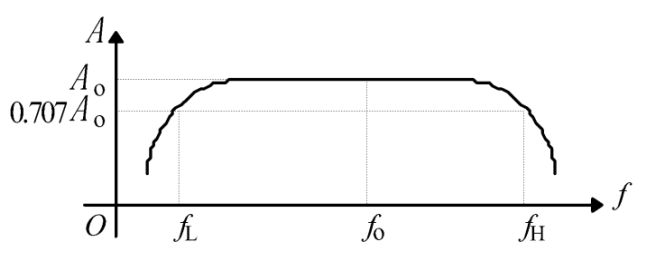
\includegraphics[width=0.6\textwidth]{ET1_9+10graph1-1.png}
				\caption{放大倍数与频率关系}
				\label{fig:fig1-1}
			\end{figure}

			\begin{enumerate}
				\item 上限频率(高频响应):
					上限频率主要受电路中的寄生电容(如晶体管的集电极-基极电容 $C_{cb}$ 和集电极-射极电容 $C_{ce}$)以及耦合电容的影响。在高频时,这些电容会形成低通滤波效应,削弱高频信号的放大能力。

					单级放大器的上限频率 $f_{H_i}$ 可以近似表示为:
					\[
					f_{H_i} \approx \frac{1}{2 \pi R_{in_i} C_{total_i}}
					\]
					其中:
					\begin{itemize}
						\item $R_{in_i}$ 是第 $i$ 级放大器的输入阻抗。
						\item $C_{total_i}$ 是第 $i$ 级放大器的总寄生电容和耦合电容。
					\end{itemize}
					
					多级放大电路的上限频率 $f_H$ 与其各级上限频率之间存在以下近似关系:
					\[
					\frac{1}{f_H} \approx 1.1 \sqrt{\frac{1}{f_{H_1}^2} + \frac{1}{f_{H_2}^2} + \cdots + \frac{1}{f_{H_n}^2}}
					\]

					在实际的多级放大电路中,当各放大级的时间常数相差悬殊时,可取起主要作用的那一级作为估算的依据。例如,若其中第 $k$ 级的上限频率 $f_{H_k}$ 比其他各级小得多时,可近似认为总的 $f_H = f_{H_k}$。


					

				\item 下限频率(低频响应):
					下限频率主要受耦合电容和旁路电容的影响。在低频时,耦合电容和旁路电容的阻抗较大,会导致信号衰减。

					单级放大器的下限频率 $f_{L_i}$ 可以近似表示为:
					\[
					f_{L_i} \approx \frac{1}{2 \pi (R_C \parallel R_{in_{next}}) C_{C_i}}
					\]
					其中:
					\begin{itemize}
						\item $R_C$ 是第 $i$ 级放大器的集电极电阻。
						\item $R_{in_{next}}$ 是下一级放大器的输入阻抗。
						\item $C_{C_i}$ 是第 $i$ 级放大器的耦合电容。
					\end{itemize}
					
					多级放大电路的下限频率 $f_L$ 与其各级下限频率之间存在以下近似关系:
					\[
					f_L \approx 1.1 \sqrt{f_{L_1}^2 + f_{L_2}^2 + \cdots + f_{L_n}^2}
					\]

					同理,若其中第 $m$ 级的下限频率 $f_{L_m}$ 比其他各级大得多时,可以近似认为总的 $f_L = f_{L_m}$。



					
			\end{enumerate}

		
		\item 静态工作点的调试方法:
			
			为了确保放大器正常工作,需要正确设置每一级放大器的静态工作点(Q点)。常用的方法有电压分压偏置和电流反馈偏置。

			\begin{enumerate}
				\item 电压分压偏置:
					
					通过分压电阻 $R_1$ 和 $R_2$ 为基极提供偏置电压:
					\[
					V_B = \frac{V_{CC} R_2}{R_1 + R_2}
					\]
					基极电流 $I_B$ 为:
					\[
					I_B = \frac{V_B - V_{BE}}{R_B + (\beta + 1) R_E}
					\]
					其中:
					\begin{itemize}
						\item $V_{BE}$ 是基-射极电压,一般约为0.7V。
						\item $R_B$ 是基极电阻。
					\end{itemize}

					集电极电流 $I_C$ 和集电极电压 $V_C$ 分别为:
					\[
					I_C \approx \beta I_B
					\]
					\[
					V_C = V_{CC} - I_C R_C
					\]

				\item 电流反馈偏置:
					
					在射极加入电阻 $R_E$ 形成电流反馈,增强稳定性。基极电压为:
					\[
					V_B = \frac{V_{CC} R_2}{R_1 + R_2}
					\]
					射极电压为:
					\[
					V_E = I_E R_E = (\beta + 1) I_B R_E
					\]
					因此基极电流为:
					\[
					I_B = \frac{V_B - V_E - V_{BE}}{R_B}
					\]

					通过调整 $R_1$、$R_2$ 和 $R_E$ 的值,可以精确调节静态工作点,确保晶体管在放大区工作。
					
			
				
			\end{enumerate}

	\end{enumerate}

	\subsubsection{负反馈放大电路}

		负反馈放大电路通过将输出信号的一部分反馈到输入端,从而改善放大器的性能。本文将总结负反馈放大电路的基本原理和作用。

		\begin{enumerate}
			\item 负反馈放大电路的基本原理:
			
				负反馈放大电路通过反馈网络将一部分输出信号反馈到输入端,用以自动调整输出电压。电压串联负反馈的基本电路如\cref{fig:fig1-2}所示,通过电阻 $R_f$ 和第一级射极电阻 $R_{e1}$ 引入交流电压串联负反馈。

				\begin{figure}[htbp]
					\centering
					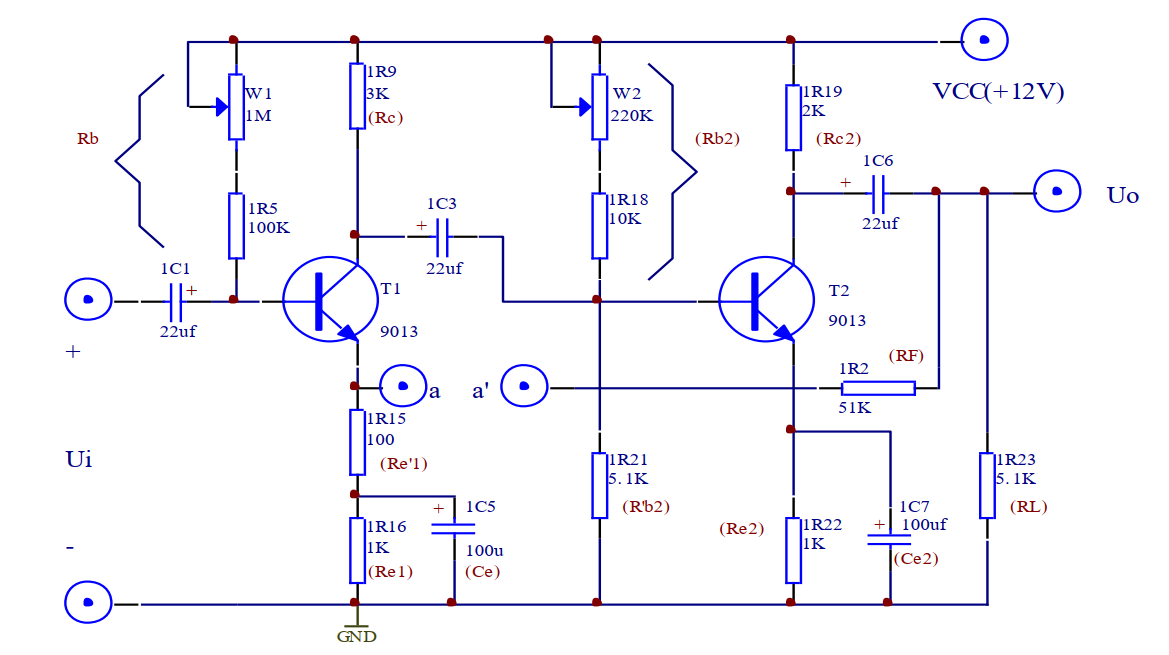
\includegraphics[width=0.8\textwidth]{ET1_9+10graph1-2.png}
					\caption{负反馈放大电路电路图}
					\label{fig:fig1-2}
				\end{figure}

				
				负反馈的作用是利用输出电压 $U_o$ 自身通过反馈网络对放大电路进行自动调整。例如,当输入电压 $U_i$ 一定时,若负载电阻 $R_L$ 减小导致输出电压 $U_o$ 下降,则电路将进行以下自动调整过程:
				\[
				R_L \downarrow \rightarrow U_o \downarrow \rightarrow U_f \downarrow \rightarrow U_{be} \downarrow \rightarrow U_o \uparrow
				\]
				
				这种反馈作用限制了 $U_o$ 的下降,从而使输出电压基本稳定。
			
			\item 负反馈的作用:
			
				负反馈在放大电路中的作用主要包括降低放大倍数、提高放大倍数的稳定性、展宽频带、减小非线性失真、抑制干扰以及改变输入输出阻抗等。

				\begin{enumerate}
					\item 降低放大器的电压放大倍数:
						引入负反馈后,反馈信号 $U_f$ 为:
						\[
						U_f = F U_o
						\]
						其中,$F$ 称为反馈系数。若原放大器的电压放大倍数为 $A_u$,加入负反馈后的电压放大倍数 $A_{uf}$ 为:
						\[
						A_{uf} = \frac{A_u}{1 + A_u F}
						\]
						其中,$1 + A_u F$ 为反馈深度。负反馈虽然使放大倍数降低,但改善了放大器的其他性能。

					\item 提高放大倍数的稳定性:
					
						负反馈可以提高放大倍数的稳定性。电源电压、负载电阻及晶体管参数的变化都会使放大器的增益发生变化,加入负反馈后可使这种变化相对变小。如果 $A_u F \gg 1$,则:
						\[
						A_{uf} \approx \frac{1}{F}
						\]
						由此可知,深度负反馈的放大器的放大倍数由反馈网络确定,而与原放大器的放大倍数无关。

					\item 展宽放大器的频带:

						负反馈可以展宽放大器的频带。阻容耦合放大器的幅频特性是中频范围放大倍数较高,高低频率两端放大倍数较低。引入负反馈后,中频段放大倍数降低较多,而高、低频段放大倍数降低较少,相当于通频带加宽了。

					\item 减小非线性失真和抑制干扰:

						负反馈可以减小放大器的非线性失真,使输出信号更接近输入信号的线性变化。此外,负反馈还可以抑制外界干扰,提高放大器的抗干扰能力。

					\item 改变放大器的输入、输出电阻:

						负反馈可以改变放大器的输入、输出电阻。例如,电压串联负反馈可以提高输入电阻,降低输出电阻,从而改善放大器的阻抗匹配性能。
				\end{enumerate}
	
		\end{enumerate}

		负反馈在放大电路中有着广泛的应用,通过降低放大倍数、提高稳定性、展宽频带、减小失真和抑制干扰等多种方式,显著改善了放大器的整体性能。
		
			
			
			
			
			
		
		
		% \item 多级放大电路的设计注意事项:
		
		% 	\begin{itemize}
		% 		\item \textbf{耦合电容的选择}:耦合电容值应适当选择,以确保所需的下限频率,同时避免过大的电容影响上限频率。
		% 		\item \textbf{阻抗匹配}:各级间的阻抗匹配要合理,避免信号反射和功率损失。
		% 		\item \textbf{温度稳定性}:采用负反馈等技术提高电路的温度稳定性,避免温漂对放大倍数的影响。
		% 		\item \textbf{电源去耦}:在电源端加入去耦电容,滤除电源噪声,确保电路稳定工作。
		% 	\end{itemize}


		% 通过上述方法和技巧,可以设计出性能良好的多级阻容耦合放大器,实现对信号的有效放大。

	
	% ---
	
	
	
	% 实验前思考题
	\subsection{实验预习题}
	
	
	% 思考题1
	\begin{question}
		负反馈放大电路的开环等效电路的画法规则是什么?画出本实验电路的开环等效电路。
	\end{question}

		在绘制负反馈放大电路的开环等效电路时,需要遵循以下规则:

		\begin{enumerate}
			\item 断开反馈回路:将反馈网络从电路中断开,使得放大器变成开环状态。
			\item 保持信号源连接:保留原信号源和放大器的输入连接,保持输入条件不变。
			\item 处理反馈网络:将反馈网络的输入端(原来连接到放大器输出的端子)接地,输出端(原来连接到放大器输入的端子)作为新的输入。
			\item 保持其他电路元件和参数:除了反馈网络,其余电路元件和参数保持不变。
		\end{enumerate}

		\cref{fig:fig1-1a}是本实验的开环等效电路:

		\begin{figure}[htbp]
			\centering
			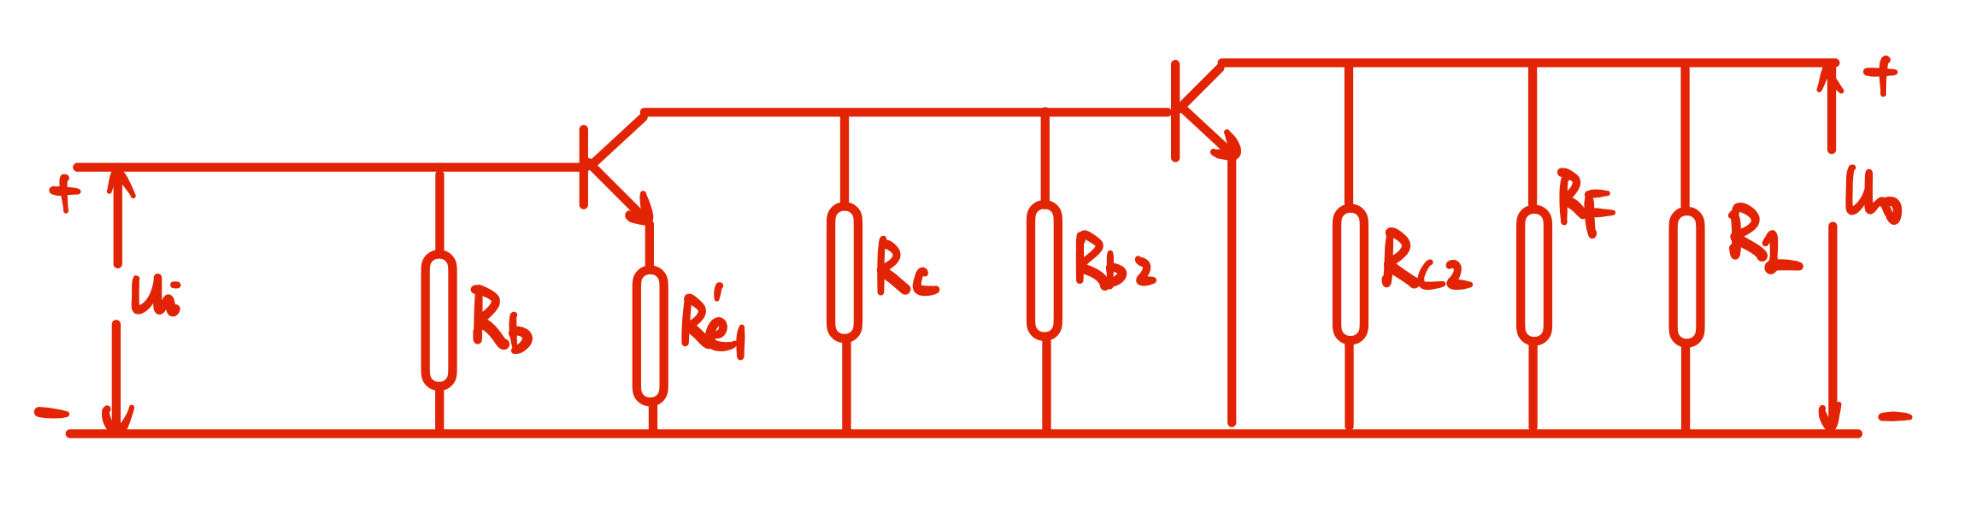
\includegraphics[width=0.8\textwidth]{graph1-1.jpg}
			\caption{开环等效电路}
			\label{fig:fig1-1a}
		\end{figure}
		




	% 思考题2
	\begin{question}
		负反馈对输入输出电阻的影响如何?根据本实验电路,给出测量其开环、闭环输入、输出电阻的实验步骤。
	\end{question}
	
		\begin{enumerate}
			\item 	输入电阻影响: 负反馈可以降低放大器的输入电阻。当负反馈应用于放大器时,反馈网络中的电压将与输入信号相反,这会导致输入电阻减小。这是因为反馈网络向输入信号源提供了一个补偿电流,从而降低了整体输入电阻。
			\item 	输出电阻影响: 负反馈可以降低放大器的输出电阻。在负反馈中,输出端的反馈信号会与输出信号相反,这会导致输出电阻减小。因为负反馈减小了输出端的电压波动,使得输出端更容易驱动负载,并且输出电阻对外部电路的影响更小。

		\end{enumerate}

		总的来说,负反馈通过降低输入和输出电阻,使得放大器更容易与外部电路匹配,并提高了整体电路的稳定性和性能。\\


		下面给出测量其开环、闭环输入、输出电阻的实验步骤。
		\begin{enumerate}
			\item 测量开环输入电阻:

				将实验电路的输入端口开路,即断开输入信号源。
				将一个标准电阻连接到输入端口,并测量输入端口的电压。
				计算输入电阻为实际输入电压与标准电阻阻值之比。

			\item 测量闭环输入电阻:

				将实验电路的输入端口接上输入信号源。
				测量输入信号源的电压和输入端口的电流。
				计算闭环输入电阻为实际输入电压与输入端口电流之比。

			\item 测量开环输出电阻:

				将实验电路的输出端口开路,即断开负载。
				施加一个小的交流信号到输入端口,并测量输出端口的电压。
				计算开环输出电阻为实际输出电压与施加信号电流之比。

			\item 测量闭环输出电阻:

				将实验电路的输出端口接上负载。
				施加一个小的交流信号到输入端口,并测量输出端口的电压和负载电流。
				计算闭环输出电阻为实际输出电压与负载电流之比。
		\end{enumerate}


		




	% 思考题3
	\begin{question}
		本实验电路中引入了哪些反馈?分析它们的组态和对放大器性能的影响。
	\end{question}
	
		引入了电压负反馈。

		\begin{enumerate}
			\item 稳定性提高: 通过降低电路的电压放大倍数,负反馈使得放大器的输出电压更加稳定。即使负载电阻发生变化,输出电压也会被调整以使得输入信号和反馈信号之间的比值保持稳定。
			\item 带宽增加: 负反馈通常可以增加放大器的带宽,因为它降低了放大器的增益,使得放大器的频率响应更平坦。
			\item 谐波失真减小: 负反馈可以减小放大器的谐波失真,使得输出信号更接近输入信号的形状。
			\item 输入/输出阻抗影响: 负反馈可以降低放大器的输入和输出阻抗,使得放大器更容易驱动负载并更容易与外部电路匹配。

		\end{enumerate}
	
		总的来说,引入电压负反馈可以改善放大器的线性度、稳定性和频率响应,从而提高整体性能。



	% ---
	
	
	
	% 实验记录	
	\clearpage
	
	% 顶栏
	\begin{table}
		\renewcommand\arraystretch{1.7}
		\centering
		\begin{tabularx}{\textwidth}{|X|X|X|X|}
			\hline
			专业: & 物理学 & 年级: & 2022级 \\
			\hline
			姓名: & 戴鹏辉\&杨舒云 & 学号: & 22344016\&22344020\\
			\hline
			室温: & 26℃  & 实验地点: & A522 \\
			\hline
			学生签名:& 见\textbf{附件}部分 & 评分: &\\
			\hline
			实验时间:& 2024/5/8\&15 & 教师签名:&\\
			\hline
		\end{tabularx}
	\end{table}
	% ---
	
	% 小标题
	\section{ET9+10 \quad 两级阻容耦合放大电路\&负反馈放大电路  \quad\heiti 实验记录}
	% ---
	
	% 实验过程记录
	\subsection{实验内容、步骤与结果}
	
	%
	\subsubsection{操作步骤记录}
		
		\begin{itemize}
			\item 两级阻容耦合放大电路实验:
			
				按电路图\cref{fig:fig1-3t}连接电路。

				\begin{figure}[htbp]
					\centering
					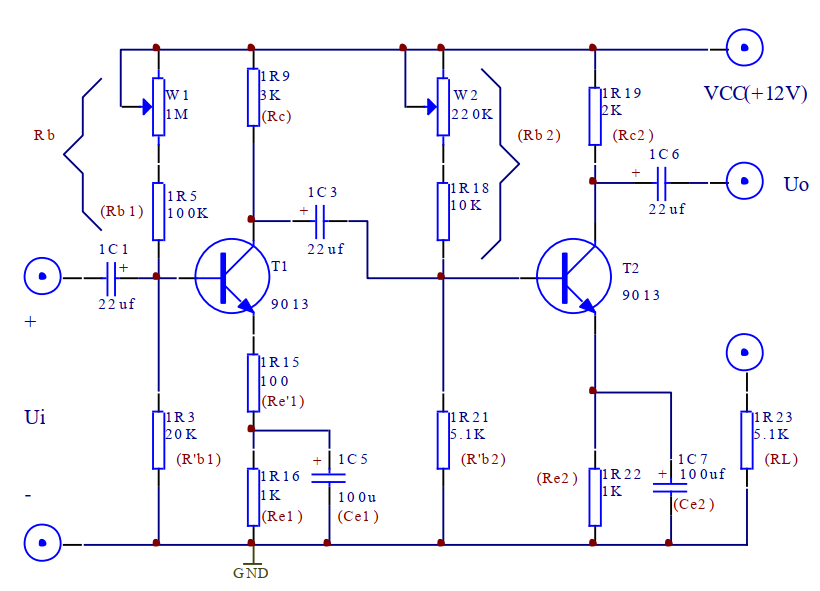
\includegraphics[width=0.8\textwidth]{ET1_9+10graph1-3.png}
					\caption{两级阻容耦合放大电路电路图}
					\label{fig:fig1-3t}
				\end{figure}


				\begin{enumerate}
					\item 调整静态工作点:
						\begin{enumerate}
							\item \textbf{调节电源电压:}
							\begin{enumerate}
								\item 将电源电压调到 $V_{CC} = 12V$。
							\end{enumerate}
						
							\item \textbf{调节电位器:}
							\begin{enumerate}
								\item 调节电位器 RW1,使得 $U_{C1}$ 在 $9 \sim 10V$ 之间。
								\item 调节电位器 RW2,使得 $U_{C2}$ 在 $6 \sim 7V$ 之间。
							\end{enumerate}
						
							\item \textbf{输入信号:}
							\begin{enumerate}
								\item 给放大器输入一个频率为 1KHz,幅度为 2mV 的信号。
							\end{enumerate}
						
							\item \textbf{观察输出波形:}
							\begin{enumerate}
								\item 使用示波器分别观察第一级和第二级放大器的输出波形。
								\item 如果输出波形有失真,可以微调电位器 RW1 和 RW2,直到两级放大器的输出信号波形都没有失真为止。
							\end{enumerate}
						
							\item \textbf{测量电位:}
							\begin{enumerate}
								\item 测量晶体管 T1 和 T2 各极的电位,并记录数据。
							\end{enumerate}
						\end{enumerate}

					
					\item 测量电压放大倍数:
					
						输入信号仍为 f=lKHz、 2mV 交流信号,在不失真的情况下,按给定的条件,分别测量放大器的第一级和第二级的输出电压 $U_{O1}$, $U_O$,记录数据。


					\item 用逐点测量法测试放大器幅频特性:
					
						\begin{enumerate}
							\item \textbf{保持输入信号:}
							\begin{enumerate}
								\item 将输入信号 $U_i = 2\text{mV}$ 保持不变。
								\item 接入负载 $R_L = 5.1\text{K}$。
							\end{enumerate}
						
							\item \textbf{逐点测量法:}
							\begin{enumerate}
								\item 改变频率,测出相应的输出电压 $U_O$。
								\item 将测量的数据记入表 9-3 中。
							\end{enumerate}
						
							\item \textbf{确定截止频率和带宽:}
							\begin{enumerate}
								\item 找出上限截止频率 $f_H$ 和下限截止频率 $f_L$(增益下降到中频增益的 0.707 倍时所对应的频率点,即 3 分贝点)。
								\item 计算放大器的带宽,$BW = f_H - f_L$。
							\end{enumerate}
						\end{enumerate}


				\end{enumerate}


			\item 负反馈放大电路实验:
				
				\begin{figure}[htbp]
					\centering
					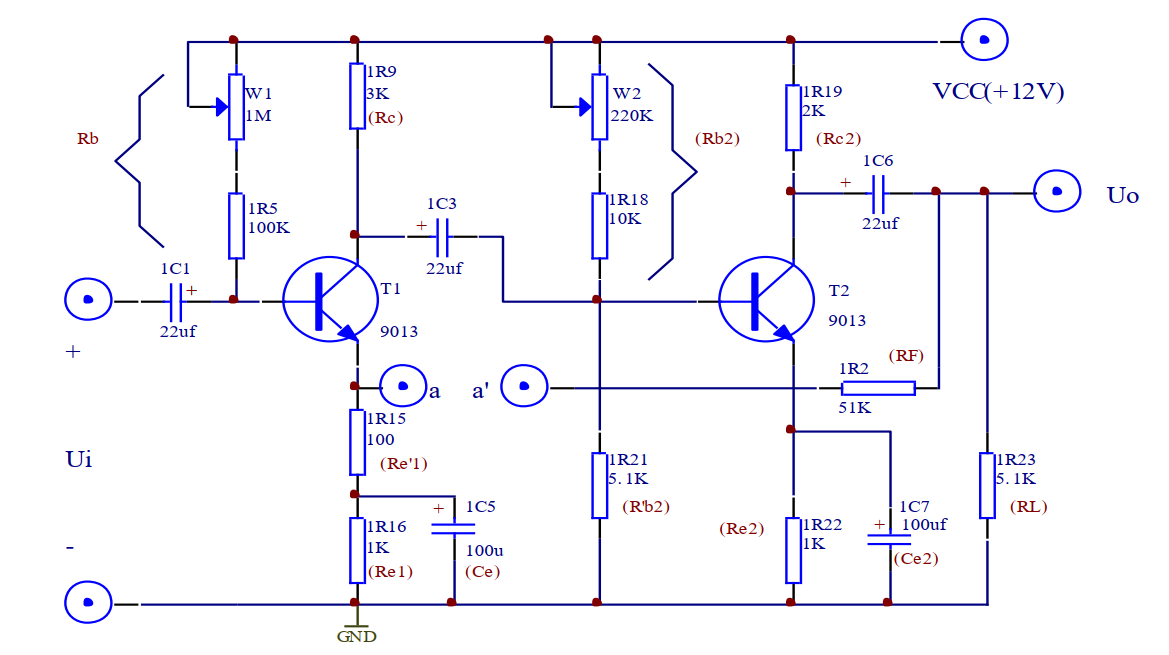
\includegraphics[width=0.8\textwidth]{ET1_9+10graph1-2.png}
					\caption{负反馈放大电路电路图}
					\label{fig:fig1-2t}
				\end{figure}

				\begin{enumerate}
					\item 调节静态工作点:
						
						按电路图\cref{fig:fig1-2t}连接电路,连接 a 和 a' 点使放大器处于闭环工作状态。将输入端对地短路($U_i = 0$),经检查无误后,接通电源。调整 W1 和 W2,使 $I_{C1} = I_{C2} = 2$ mA。测量各级静态工作点,并记录数据。


					\item 观察负反馈对放大倍数的影响:
					
						在输入端加入 $U_i = 2$ mV、$f = 1$ kHz 的正弦信号,分别测量电路在开环(a 与 a' 断开且将 a' 接地)与闭环(a 与 a' 点连接)工作时的输出电压 $U_O$,同时用示波器观察输出波形,注意波形是否失真。计算电路在开环与闭环工作时的电压放大倍数,记录数据,并验证理论公式的正确性。


					\item 观察负反馈对放大倍数稳定性的影响:
					
						将电源电压从 12V 调到 10V,在输入端加入 $U_i = 2$ mV、$f = 1$ kHz 的正弦波信号,分别测量电路在开环与闭环工作状态时的输出电压,注意波形是否失真。计算电压放大倍数的相对变化量,记录数据,并验证理论公式的正确性。


					\item 幅频特性测量:
					
						在电源电压 $V_{CC} = 12V$(不接负载)情况下,在输入端加入 $U_i = 2$ mV、$f = 1$ kHz 的正弦波信号。然后调节信号源频率使 $f$ 下降(保持 $U_i$ 不变),测量 $U_o$,在电压放大倍数下降到中频电压放大倍数的 0.707 倍时所对应的频率点附近多测几点,找出下限频率。同理,使 $f$ 上升,找出上限频率,求出放大器的带宽 $BW = f_H - f_L$,并对开环、闭环状态进行比较。


					\item 用示波器观察负反馈对放大器非线性失真的改善:
					
						在上述实验基础上,将信号频率设为 1kHz。当放大器处于开环状态时,适当加大输入信号,使输出电压波形出现轻度非线性失真,观察并绘出输出电压波形。在放大器处于闭环状态时,适当加大输入信号,使输出信号幅值接近开环时的输出信号失真波形幅度,观察并绘出输出电压波形,并对开环和闭环状态进行比较。

				\end{enumerate}
			

		\end{itemize}	
	
	%
	\subsubsection{实验结果记录}

	\begin{itemize}
		\item 两级阻容耦合放大电路实验:
		
			\begin{enumerate}
				\item 调整静态工作点:
					
					如\cref{tbl:table1}所示:

					\begin{table}[htbp]
						\centering
						\begin{tblr}{
						cells = {c},
						cell{1}{1} = {c=3}{},
						cell{1}{4} = {c=3}{},
						vline{1,4,7} = {1}{},
						vline{1,4,7} = {2-3}{},
						hline{1-2,4} = {-}{},
						}
						$T_1$    &       &       & $T_2$    &       &       \\
						$U_{C1}$/V & $U_{B1}$/V & $U_{E1}$/V & $U_{C2}$/V & $U_{B2}$/V & $U_{E2}$/V \\
						9.855 & 1.586 & 0.98  & 7.651 & 2.44  & 1.815 
						\end{tblr}
						\caption{两级阻容耦合放大电路静态工作点设置}
						\label{tbl:table1}
					\end{table}
				
				\item 测量电压放大倍数:
				

					如\cref{tbl:table2}所示:

					\begin{table}[htbp]
						\centering
						\begin{tblr}{
						cells = {c},
						vline{1-2,5,8} = {-}{},
						hline{1-2,4} = {-}{},
						}
									& $U_i$/mV & $U_{o1}$/mV & $U_o$/V & $A_{u1}$  & $A_{u2}$      & $A_u$   \\
						放大器空载        & 2     & 25.6   & 2.48 & 12.8 & 96.875   & 1240 \\
						$R_L=5.1K\Omega$ & 2     & 25.8   & 2.13 & 12.9 & 82.55814 & 1065 
						\end{tblr}
						\caption{两级阻容耦合放大电路放大倍数测量}
						\label{tbl:table2}
					\end{table}


				\item 用逐点测量法测试放大器幅频特性:
				
					如\cref{tbl:table3}所示:
					
					\begin{table}[htbp]
						\centering
						\begin{tblr}{
						vline{1-2,12} = {-}{},
						hline{1,3} = {-}{},
						}
						f/Hz  & 45   & 55   & 60   & 100 & 300  & 600 & 1000 & 3000 & 6000 & 8000 \\
						$U_o$/mV & 1.14 & 1.22 & 1.28 & 1.4 & 1.66 & 1.7 & 1.72 & 1.53 & 1.21 & 1.12 
						\end{tblr}
						\caption{两级阻容耦合放大电路幅频特性测量}
						\label{tbl:table3}
					\end{table}


			\end{enumerate}


		\item 负反馈放大电路实验:
			
			\begin{enumerate}

				\item 调节静态工作点:
					
					如\cref{tbl:table4}所示:

					\begin{table}[H]
						\centering
						\begin{tblr}{
						vline{1,4,7} = {-}{},
						hline{1,3} = {-}{},
						}
						$U_{C1}$/V & $U_{B1}$/V & $U_{E1}$/V & $U_{C2}$/V & $U_{B2}$/V & $U_{E2}$/V \\
						5.784 & 3.504 & 2.874 & 6.102 & 3.087 & 2.45  
						\end{tblr}
						\caption{负反馈放大电路静态工作点设置}
						\label{tbl:table4}
					\end{table}
					
					

				\item 观察负反馈对放大倍数的影响:
					
					实验中选用信号发生器$V_{rms}=2mV$,结果如\cref{tbl:table5}所示:	

					\begin{table}[H]
						\centering
						\begin{tblr}{
						cells = {c},
						cell{2}{2} = {r=2}{},
						vline{1,3,5} = {1-2}{},
						vline{1,3,5} = {3}{},
						hline{1-2,4} = {-}{},
						}
						& $U_i$  & $U_o$    & $A_u$  \\
						开环 & 2mV & 1.9V  & 950 \\
						闭环 &     & 149mV & 75  
						\end{tblr}
						\caption{负反馈对放大倍数的影响测量}
						\label{tbl:table5}
					\end{table}
					

				\item 观察负反馈对放大倍数稳定性的影响:
				
					实验中选用信号发生器$V_{rms}=2mV$,结果如\cref{tbl:table6}所示:

					\begin{table}[htbp]
						\centering
						\begin{tblr}{
						cells = {c},
						cell{1}{2} = {c=2}{},
						cell{1}{4} = {c=2}{},
						vline{1-3,5,6} = {1}{},
						vline{1-2,4,6} = {2-4}{},
						hline{1,3,5} = {-}{},
						hline{2} = {2-5}{},
						}
						& $V_{cc}$=12V &      & $V_{cc}$=10V &     \\
						& $U_o$      & $A_u$   & $U_o$      & $A_u$  \\
						开环 & 1.56V   & 780  & 1.46V   & 730 \\
						闭环 & 143mV   & 71.5 & 142mV   & 71  
						\end{tblr}
						\caption{负反馈放大电路负反馈对放大倍数稳定性的影响测量}
						\label{tbl:table6}
					\end{table}

				\item 幅频特性测量:
				
					实验中选用信号发生器$V_{pp}=2mV$,结果如\cref{tbl:table7-1},\cref{tbl:table7-2}所示:
					
					\begin{table}[htbp]
						\begin{minipage}{.5\linewidth}
							\centering
							\begin{tabular}{|ll|} 
								\hline
								f/Hz  & Uo/V  \\ 
								\hline
								80    & 2.12  \\
								83    & 2.16  \\
								85    & 2.20  \\
								90    & 2.24  \\
								95    & 2.30  \\
								100   & 2.34  \\
								200   & 2.74  \\
								400   & 2.94  \\
								600   & 3.02  \\
								800   & 3.04  \\
								1000  & 3.04  \\
								2000  & 3.04  \\
								4000  & 2.94  \\
								5000  & 2.82  \\
								6000  & 2.82  \\
								7000  & 2.76  \\
								8000  & 2.66  \\
								9000  & 2.62  \\
								10000 & 2.50  \\
								11000 & 2.48  \\
								12000 & 2.40  \\
								13000 & 2.32  \\
								14000 & 2.24  \\
								15000 & 2.20  \\
								15500 & 2.18  \\
								16000 & 2.12  \\
								17000 & 2.06  \\
								\hline
							\end{tabular}
							\caption{负反馈放大电路幅频特性测量(开环)}
							\label{tbl:table7-1}
						\end{minipage}%
						\begin{minipage}{.5\linewidth}
							\centering
							\begin{tabular}{|ll|}
								\hline
								f/Hz & Uo/mV \\
								\hline
								30 & 39.96 \\
								40 & 46.79 \\
								50 & 50.93 \\
								70 & 54.82 \\
								100 & 57.96 \\
								200 & 59.74 \\
								500 & 61.09 \\
								1000 & 61.30 \\
								2000 & 61.51 \\
								5000 & 61.23 \\
								10000 & 61.15 \\
								20000 & 60.99 \\
								50000 & 60.89 \\
								80000 & 60.64 \\
								90000 & 60.00 \\
								100000 & 60.04 \\
								110000 & 59.80 \\
								120000 & 59.50 \\
								130000 & 58.80 \\
								140000 & 57.70 \\
								150000 & 57.40 \\
								160000 & 56.90 \\
								170000 & 52.62 \\
								180000 & 49.73 \\
								190000 & 42.28 \\
								\hline
							\end{tabular}
							\caption{负反馈放大电路幅频特性测量(闭环)}
							\label{tbl:table7-2}
						\end{minipage}
					\end{table}


				\item 用示波器观察负反馈对放大器非线性失真的改善:
				

				如图\cref{fig:fig2-1},\cref{fig:fig2-2}:
				\begin{figure}[htbp]
					\centering
					\includegraphics[width=0.5\textwidth]{ET1_9+10graph2-1.png}
					\caption{示波器观察负反馈对放大器非线性失真的改善1}
					\label{fig:fig2-1}
				\end{figure}


				\begin{figure}[htbp]
					\centering
					\includegraphics[width=0.5\textwidth]{ET1_9+10graph2-2.png}
					\caption{示波器观察负反馈对放大器非线性失真的改善2}
					\label{fig:fig2-2}
				\end{figure}
				
					
			\end{enumerate}
		

	\end{itemize}	
	
	% ---
	



	% 原始数据
	\clearpage
	\subsection{原始数据记录}
	实验记录本上的原始数据见\cref{fig:data1}(签字),\cref{fig:data2},\cref{fig:data3}(签字)。
		
		
		\begin{figure}[htbp]
			\centering
			\subfloat[原始数据1]
			{\includegraphics[width=0.35\textwidth]{ET1_9+10Gradata-1.jpg}\label{fig:data1}}
			\quad
			\subfloat[原始数据2]
			{\includegraphics[width=0.35\textwidth]{ET1_9+10Gradata-2.jpg}\label{fig:data2}}
			\quad
			\subfloat[原始数据3]
			{\includegraphics[width=0.35\textwidth]{ET1_9+10Gradata-3.jpg}\label{fig:data3}}
			\quad

			\caption{原始数据}
			\label{fig:original_data}
		\end{figure}


	实验台桌面整理见%\textbf{附件}部分(\cref{})。
	
	% 其它原始数据见%\cref{}。
	% ---
	
	% 问题记录
	\subsection{实验过程遇到问题及解决办法}
	\begin{enumerate}
		\item 由于两个实验不是同时进行的,两个实验的工作环境(即静态工作点)设置的不一样,所以两个实验之间的数据难以对比。
		\item 电路板上的触点较少,难以测量某些点之间的电压。
	\end{enumerate}
	% ---
	
	
	
	% 分析与讨论	
	\clearpage
	
	% 顶栏
	\begin{table}
		\renewcommand\arraystretch{1.7}
		\begin{tabularx}{\textwidth}{|X|X|X|X|}
			\hline
			专业:& 物理学 &年级:& 2022级\\
			\hline
			姓名: & 戴鹏辉\&杨舒云 & 学号:& 22344016\&22344020 \\
			\hline
			日期:& 2024/5/23 & 评分: &\\
			\hline
		\end{tabularx}
	\end{table}
	% ---
	
	% 小标题
	\section{ET9+10 \quad 两级阻容耦合放大电路\&负反馈放大电路 \ \heiti 分析与讨论}
	% ---
	
	% 数据处理
	\subsection{实验数据分析}
	
	
		
			\begin{enumerate}
				
				\item 比较电压放大倍数:
				
					\begin{itemize}
						\item 在”两级阻容耦合放大电路“实验中,测量电压放大倍数如\cref{tbl:table2}。

							可以看到,不论是在负载为空载,或是负载为$R_L=5.1k\Omega$时,两级之间的放大倍数关系均有$A_u = A_{u1} \cdot A_{u2}$,即验证了理论公式。
			
								\begin{enumerate}
									\item 放大器空载时:
			
										$A_{u1} \cdot A_{u2} = 12.8 \times 96.875 = 1240 = A_u$
			
			
									\item 放大器负载$R_L=5.1k\Omega$时:
									
										$A_{u1} \cdot A_{u2} = 12.9 \times 82.55814 = 1065 = A_u$	
								\end{enumerate}
						
						\item 在”负反馈放大电路“实验中,我们观察了负反馈对放大倍数的影响,结果如\cref{tbl:table5}。
						
								可以看到,开环状态下放大倍数为950倍,而闭环时放大倍数仅有75倍。说明负反馈会显著降低放大电路的放大倍数。因为负反馈引入了一部分输出信号反相后反馈到输入端,这会抵消一部分输入信号,从而减小整体的输出信号,导致放大倍数降低。

						\item 在”负反馈放大电路“实验中,我们还观察了负反馈对放大倍数稳定性的影响,结果如\cref{tbl:table6}。
						
								可以看到,在开环状态下,当$V_{cc}$由12V降低至10V时,放大倍数由780倍降低至730倍,有显著的变化。

								而在闭环状态下,当$V_{cc}$由12V降低至10V时,放大倍数由71.5倍变化至71倍,变化不明显。

								这说明尽管负反馈降低了放大倍数,但它显著提高了放大倍数的稳定性。这是因为负反馈能够减小放大器增益对外界条件(如温度变化、供电电压波动、器件老化等)的依赖性。负反馈引入后,放大电路的增益主要由反馈网络决定,而反馈网络的参数通常比放大元件(如晶体管)的参数更稳定和精确。
					\end{itemize}
				
				

				
			

				\item 放大器幅频特性分析:
				
					\begin{enumerate}
						\item 在“两级阻容耦合放大电路”实验中,我们使用逐点法测量了放大器的幅频特性,结果如\cref{fig:fig3_1}
						
							\begin{figure}[htbp]
								\centering
								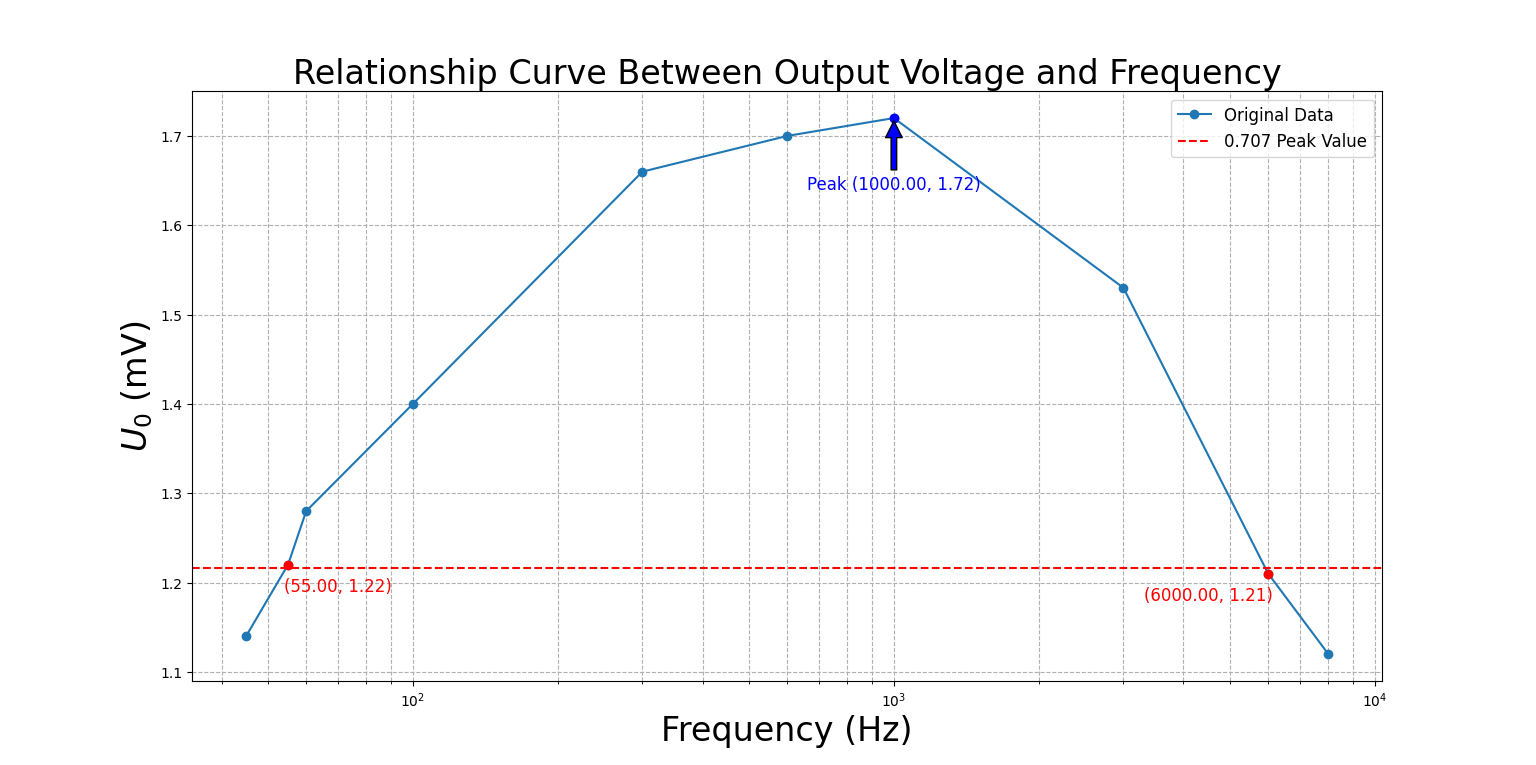
\includegraphics[width=1\textwidth]{graph3_1.png}
								\caption{放大器频率响应}
								\label{fig:fig3_1}
							\end{figure}

							从图中可以看出,该放大电路的频宽大约为$55Hz - 6000Hz$,超过这个频率范围后,输出电压下降至峰值的0.707倍。

						\item 在“负反馈放大电路”实验中,我们对比了开环、闭环状态下的幅频响应,如\cref{fig:fig4_1}、\cref{fig:fig4_2}:
						
							\begin{figure}[htbp]
								\centering
								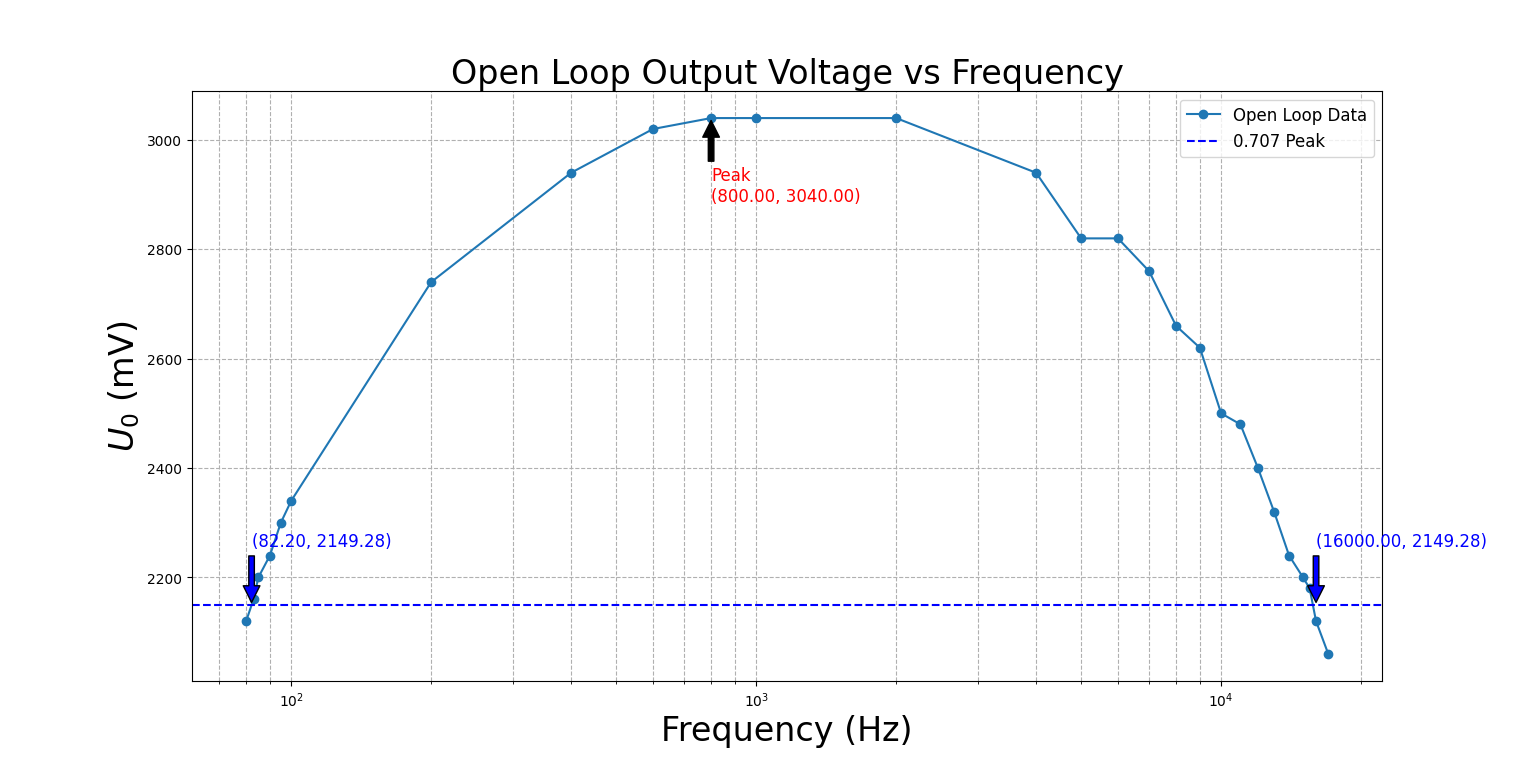
\includegraphics[width=1\textwidth]{graph4_1.png}
								\caption{开环状态频率响应}
								\label{fig:fig4_1}
							\end{figure}

							\begin{figure}[htbp]
								\centering
								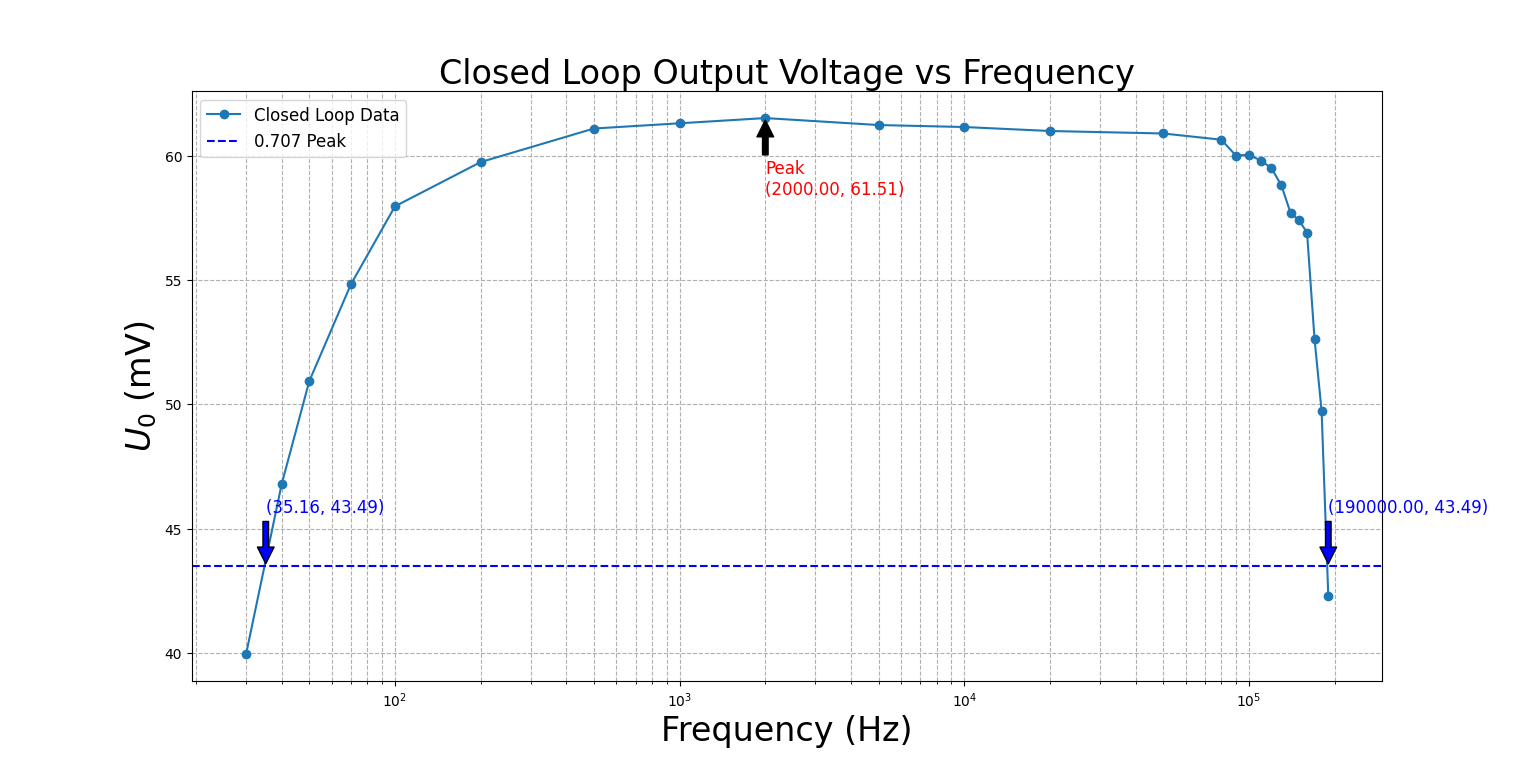
\includegraphics[width=1\textwidth]{graph4_2.png}
								\caption{闭环状态频率响应}
								\label{fig:fig4_2}
							\end{figure}

							带宽分别为:
								\begin{itemize}
									\item 开环:$BW = f_H - f_L = 16000 - 82 Hz = 15918Hz$
									\item 闭环:$BW = f_H - f_L = 19000 - 35 Hz = 18956Hz$
								\end{itemize}

							分析:
									\begin{enumerate}
										\item 开环状态的影响
											
											\begin{itemize}
												\item 高增益:在开环状态下,放大器的增益非常高。这意味着即使输入信号非常小,输出信号也会被大幅度放大。然而,这种高增益也容易导致失真,因为一旦输入信号达到某个水平,放大器就会开始饱和,导致输出信号失真。
												\item 灵敏度高:由于高增益,放大器对输入信号的变化非常敏感。这种灵敏度意味着放大器在处理高频信号时可能会引入更多的噪声和失真。
												\item 带宽较窄:开环状态下,放大器的带宽通常较窄。在高增益的情况下,放大器的频率响应范围受到限制,导致放大器只能在相对较窄的频率范围内保持有效增益。
											\end{itemize}
										
										\item 闭环状态的影响
										
											\begin{itemize}
												\item 降低增益:在闭环状态下,负反馈降低了系统的整体增益。虽然这意味着输出信号的幅度相对于开环状态会减小,但这种降低增益的效果也减小了失真,因为放大器在处理较大振幅的输入信号时不会轻易饱和。
												\item 稳定性增强:负反馈提高了放大器的稳定性,使得放大器对输入信号的变化不那么敏感。这减少了噪声和其他干扰对输出信号的影响,提高了放大器的线性度和稳定性。
												\item 带宽增大:负反馈的应用扩大了放大器的带宽,使得放大器能够在更宽的频率范围内保持有效增益。这使得放大器在处理高频信号时具有更好的性能。
											\end{itemize}
								
										\item 总结
										
											在开环状态下,放大器具有高增益和高灵敏度,但带宽较窄,容易导致信号失真。而在闭环状态下,负反馈降低了增益,提高了稳定性,显著扩大了带宽,使放大器能够处理更大振幅的输入信号而不至于失真。因此,负反馈放大器在闭环状态下具有更好的性能,能够在更宽的频率范围内稳定工作,处理更大振幅的输入信号而保持线性响应。
									\end{enumerate}
							
					\end{enumerate}
					
				\item 观察负反馈对放大器非线性失真的改善:
					
					由\cref{fig:fig2-1}、\cref{fig:fig2-2}可以看到


						\begin{enumerate}
							\item 降低失真
							\begin{enumerate}
								\item 负反馈通过将部分输出信号反馈到输入端并与输入信号相减,减小了放大器的增益。这种增益的降低使得放大器在处理较大振幅输入信号时不容易达到饱和状态,从而减少了失真。
								\item 负反馈放大器的输出信号更接近理想的线性响应,因为负反馈可以补偿放大器内部的非线性成分,降低非线性失真。
							\end{enumerate}
							
							\item 增加线性度
							\begin{enumerate}
								\item 负反馈提高了放大器的线性度,使输出信号更准确地跟随输入信号的变化。这意味着放大器的输出信号会更加精确和稳定,减少了由非线性引起的谐波失真和互调失真。
							\end{enumerate}
					
							\item 改善频率响应
							\begin{enumerate}
								\item 负反馈扩大了放大器的频率响应范围,使得放大器在更宽的频率范围内保持较低的失真。这对高频和宽带应用特别重要,因为这些应用要求放大器在整个频率范围内保持低失真。
							\end{enumerate}
					
							\item 降低噪声
							\begin{enumerate}
								\item 负反馈还可以减小噪声对信号的影响,提高信噪比,从而进一步改善放大器的整体性能和输出信号的质量。
							\end{enumerate}
						\end{enumerate}
				
					


				


				


					
			\end{enumerate}
		


	
	% ---
	

	\clearpage

	% 实验后思考题
	\subsection{实验后思考题}
	
	%思考题1
	\begin{question}
		如何增加阻容耦合放大器的频率范围?
	\end{question}
	
		\begin{enumerate}
			\item \textbf{增加阻容耦合放大器的频率范围的方法}
			\begin{enumerate}
				\item 选择合适的耦合电容和旁路电容
				\begin{enumerate}
					\item 耦合电容:选择较大的耦合电容可以降低低频截止频率,从而扩展低频响应。
					\item 旁路电容:选择合适的旁路电容可以提高高频响应,扩展高频带宽。
				\end{enumerate}
				
				\item 优化放大器的输入和输出电阻
				\begin{enumerate}
					\item 降低输入电阻:通过选择低输入电阻的放大器或增加输入端的缓冲器来提高高频响应。
					\item 减小输出电阻:通过选择具有低输出电阻的放大器或增加输出端的缓冲器来提高高频响应。
				\end{enumerate}
		
				\item 提高放大器的增益带宽积(GBW)
				\begin{enumerate}
					\item 选择高GBW的运算放大器:选择具有高GBW的运算放大器可以提高整个电路的频率范围。
					\item 多级放大:采用多级放大电路,每一级放大器的增益较低但频率范围较宽,组合起来可以实现高增益和宽频带。
				\end{enumerate}
		
				\item 改进电路布局和布线
				\begin{enumerate}
					\item 减少寄生电容和电感:通过优化电路布局、缩短高频信号的路径以及减少相邻导线间的电容耦合,可以减小寄生效应,提高高频带宽。
					\item 使用屏蔽和接地:在高频电路中,使用屏蔽和良好的接地可以减少噪声和干扰,提高信号完整性,扩展频率范围。
				\end{enumerate}
		
				\item 温度补偿和稳定性设计
				\begin{enumerate}
					\item 温度补偿:通过设计温度补偿电路,可以保持频率响应的稳定,从而扩展频率范围。
					\item 稳定性设计:使用补偿电容和适当的反馈网络可以提高稳定性,防止自激振荡。
				\end{enumerate}
			\end{enumerate}
		\end{enumerate}


	% 思考题2
	% \begin{question}
		
	% \end{question}
	
	% % 思考题3
	% \begin{question}
		
	% \end{question}
	
	% ---
	
	
	% 结语部分
	\clearpage
	
	% 小标题
	\section{ET9+10 \quad 两级阻容耦合放大电路\&负反馈放大电路 \quad\heiti 结语}
	% ---
	
	% 总结、杂谈与致谢
	% \subsection{实验心得和体会、意见建议等}
	% \begin{enumerate}
	% 	\item 
	% \end{enumerate}
	% ---
	
	% 参考文献
	\subsection{参考文献}
	[1] 维基百科 https://zh.wikipedia.org
	
	[2] 沈韩.基础物理实验.——北京:科学出版社,2015.2 ISBN:978-7-03-043311-4
	
	% ---
	
	% 附件
	\subsection{附件及实验相关的软硬件资料等}
	试验台桌面整理如%\cref{}所示。
	
	实验报告个人签名如\cref{fig:name}。
	
	\begin{figure}[htbp]
		\centering
		\subfloat[]{
			
\includegraphics[width=0.45\textwidth]{name.png}
		}
		\subfloat[]{
			
\includegraphics[width=0.45\textwidth]{name-TaLEs.jpg}
		}
		\caption{个人签名}
		\label{fig:name}			
	\end{figure}
	
	% ---
	
	相关代码已上传至Github。
	
	
	
\end{document}